% --------------------------------------------------------------------

\chapter[Explosive Transients]{Explosive Transients}
\def\chpname{transients}\label{chp:\chpname}

% \noindent {\it
% Mike Lund, Ashish Mahabal, Stephen Ridgway, Lucianne Walkowicz, Rahul Biswas, Michelle Lochner, Jeonghee Rho, Eric Bellm...
% }

Chapter editors:
\credit{ebellm}?,
\credit{fedhere}?,


% --------------------------------------------------------------------

\section{Introduction}

Explosive transients such as novae, supernovae (SNe), and gamma-ray bursts (GRBs) probe the final stages of stellar evolution.
Cadence choices are vital to determining LSST's ability to discover and characterize these events.
Different types and time scales of phenomena benefit from different sampling strategies---sometimes significantly different.  Competing objectives described in this chapter are at the heart of LSST observing strategy and cadence design.

When evaluating a particular observation or series of observations in light of how they perform for a specific science case, it may be helpful to think of metrics as lying along a continuum between discovery and characterization. Discovery requires a minimum amount of information to recognize an event or object as a candidate of interest, which necessarily involves some level of bare-bones characterization (upon which said recognition is based); rich characterization, on the other hand, implies that an event may not only be recognized as a candidate of interest, but basic properties of the event or object may be determined from the observation (e.g. including but not limited to classification of the event). The interpretation of a given metric along this continuum has implications for the subsequent action and analysis required, particularly as regards possible follow-up observations with other facilities.

In this chapter we focus on LSST's potential to advance the science of transients as astrophysical objects; the use of SNe for cosmology is discussed in \autoref{chp:cosmo}.

% --------------------------------------------------------------------

\section{Transient Events}
\def\secname{\chpname:transients}\label{sec:\secname}

\credit{StephenRidgeway},
\credit{AshishMahabal},
\credit{ohadshemmer}

Transient events may benefit from substantial temporal sampling
(matched to the time constant of the event) with color information
(perhaps contemporaneous) to support characterization and
classification, obtained over the limited duration of interest.
Transient events slower than $\sim$ weeks may be adequately sampled by
a uniform LSST cadence.  Faster events may require special scheduling
strategies.  For some event types, LSST can only be expected to
provide a discovery service, and followup will necessarily be
performed elsewhere.

% --------------------------------------------------------------------

\subsection{Targets and Measurements}
\label{sec:\secname:targets}

The class of transients includes a heterogeneous assortment of objects and phenomena.

\begin{center}
\begin{tabular}{| p{3cm} | p{8cm} | l | l |}
\hline Transient Type & Examples of target science & Amplitude & Time Scale\\
\hline
Flare stars & Flare frequency, energy, stellar age & large & min\\
Cataclysmic variables  & Interacting binaries, stellar evolution, compact objects, explosive events & small & min\\
Supernovae & SN physics, mass loss, distance scale, cosmology& large & days\\
Active galactic nuclei & Galaxy evolution, reverberation mapping, black hole physics& large & weeks\\
Stellar microlensing & Exoplanet statistics& large & hours\\
Gamma ray bursts & Optical discovery and characterization& large & min\\
LIGO detections & Source position and characterization& unknown & min\\
Serendipity & Discovery and characterization& unknown & unknown\\
Tidal Disruption Events & Discovery and characterization & large & days\\
 \hline \end{tabular}
 \end{center}

Among the targets in this list, only AGN are likely to be sampled with sufficient resolution by a uniform LSST cadence - in fact for AGN, a challenge may be to spread visits sufficiently in time to avoid excessive seasonal gaps.

For very short lived phenomena (stellar flares, CV outbursts, GRBs, LIGO events) it appears that the function of LSST will be to provide discoveries and/or simple characterization.  Followup to discovery/identification, if required, will surely take place elsewhere.

For events requiring intensive monitoring (stellar microlensing, exoplanet transits), the followup will certainly take place elsewhere.

Supernovae fall in an intermediate time range.  LSST will provide multiple visits in multiple filters during the typical SN duration.  This sampling may be insufficient for many (including key) science objectives.  However, a moderate, and feasible, change to LSST observing strategy, may enhance the sampling for part of the sky part of the time, greatly enhancing the usefulness of SN observations.

For Tidal Disruption Events, where the fading time-scale is much more gradual (over weeks to months) than the rise time-scale it will be worth checking - through a metric - how many will be missed (as alerts). Ref. Science Book: 10.6.1. Also ref. recent papers.

Serendipitous discoveries are of course harder to plan for.  An ideal transient discovery survey would include heavy coverage of all time scales. LSST will cover longer time periods well, but will have to make some choices of emphasis in coverage of shorter time-scales.


% --------------------------------------------------------------------

\subsection{Metrics}
\label{sec:\secname:metrics}

\begin{center}
\begin{tabular}{| p{5cm} |p{10cm} |}
\hline Metric & Description\\
\hline
SNe & Number of events adequately sampled\\
Serendipity & Histogram of median visit series length vs maximum visit spacing within the series\\
  \hline \end{tabular}
 \end{center}

The metrics for SNe will be highly specialized and based on the best available understanding of SN light curve analysis and the expected event population.

The suggested metric set for serendipity is based on the simple-minded idea that a novel transient will be characterized by a band-limited, finite waveform, and that a useful observation series will consist of a series of samples extending over the duration of the event, with at least critical sampling of the fastest variations.  Since for some event durations the number of useful time series will be small, it may be useful to look not at the median length, but the median length of a subset size preselected as possibly useful (e.g. the$10^3$ longest series).

Lund et al. (2015; \url{http://arxiv.org/pdf/1508.03175.pdf}) discuss three metrics that have been incorporated into the MAF. Two of these metrics deal explicitly with time variable behavior: a) observational triplets, and b) detection of periodic variability.

\subsubsection{Observational triplets (TripletMetric)}

This metric provides a means of evaluating whether a transient event on some timescale of interest has been detected, by testing for a sequence of three observations. The object must be detected in quiescence, followed by two subsequent detections above some threshold; this sequence of observations allows the magnitude of the change to be measured, as well as its timescale.

This metric may be used for a variety of astrophysical phenomena, in particular transient events on variable objects (e.g. novae, stellar flares), in that it is general with respect to the amplitude of the brightness variation as well as the timescale of said change. The requirement of a detection prior to outburst does constrain it to objects that have already been detected in quiescence (in other words, not necessarily ``true'' transients), although there may be some cases where this is not the case (e.g. a supernova occurring on a previously detected galaxy). In practice, the time lapse between the first and second and second and third observations must be comparable (between 10$^2$ and 10$^5$ seconds) for discovery. This metric may be calculated for a given OpSim run and then further reduced to a histoogram in logarithmic time bins; the minimum number of bins to construct an interesting sample of objects is source-dependent.

\subsubsection{Transient Metric (transientAsciiMetric)}

Calculate what fraction of transients would be detected using an ascii input file for the lightcurve.

\subsection{Proposed Metrics}

The following is a raw list of metric ideas; these need specificity and further description.

The triplet metric may also be altered to include filter constraints, such that the triplets are drawn from a single filter or subset of filters.

Color evolution constraint: triplets of observations in a specific color (really requirement of two triplets in multiple filters)

  2D Histogram of delta t?s between observations constituting a triplet

Histogram of median visit series length vs maximum visit spacing within the series

Number of events adequately sampled

% --------------------------------------------------------------------

\subsection{OpSim Analysis}
\label{sec:\secname:analysis}

Analysis shows that current simulations provide  poor coverage in any one filter for transient events longer than a deep drilling session ($\sim$30 minutes) and shorter than $\sim$ weeks.

Simulated performance for SN observations must be analyzed for both main survey and mini-survey (deep drilling) productivity.  It is considered that current simulated schedules give inadequate performance for SN science.



% --------------------------------------------------------------------

\subsection{Discussion}
\label{sec:\secname:discussion}

Community studies are providing improving SNe metrics, and continuing communication between the SN and LSST communities is essential to tuning the observing strategy to deliver the SN time series that are needed and possible.

Improving LSST science return for SNe will also improve sampling of all transients with similar or somewhat shorter characteristic times.  Non-uniform survey strategies (rolling cadence) can significantly improve the LSST performance for faster transients.  Interpretation of multiple filters for novel events may be powerful, or problematic, since color may be uncertain.

Some insight into fast transients may be available from image pairs  or triples (as opposed to more complete series).  These include the pair of images in a visit - which could be useful in studying the rise time of an extremely fast event.  This includes the characteristic grouping of visits (typically 0.5 to 1.0 hour separation) planned for purposes of identifying asteroids.  It also includes fortuitous multiple sampling due to field overlap, providing additional sampling, which may be random or systematic, depending on the scheduling, on a time scale of minutes to hours.  The sampling benefits of this fortuitous overlap have not yet been investigated.


\navigationbar

% --------------------------------------------------------------------

% ====================================================================
%+
% SECTION:
%    gw.tex
%
% CHAPTER:
%    transients.tex
%
% ELEVATOR PITCH:
%-
% ====================================================================

\section{Gravitational Wave Sources}
\def\secname{\chpname:gw}\label{sec:\secname}

\credit{raffaellamargutti},
\credit{Doctor},
\credit{Fong},
\credit{Haiman},
\credit{Kalogera},
\credit{Trimble},
\credit{Zauderer}

The first detection of Gravitational Waves (GW) by the advanced
LIGO/Virgo collaboration \citep{Abbott16, Abbott09, Acernese08} has
recently opened a new window of exploration into our Universe. The
amount of information that can be revealed by the properties of the GW
emission is immense and holds promises for revolutionary insights,
including accurate masses and spins of neutron stars and black holes,
tests of General Relativity and an accurate census of the neutron star
(NS) and black hole (BH) populations that might challenge our current
understanding of massive stellar evolution. However, GW events are
poorly localized (10-100 deg$^2$ at the time of LSST operations). The
identification of EM counterparts would provide precise localization and
distance measurements, in addition to the necessary astrophysical
context (e.g. host galaxy properties, connection to specific stellar
populations) to fully exploit the revolutionary power of this new GW
era.

% --------------------------------------------------------------------

\subsection{Target measurements and discoveries}
\label{sec:\secname:targets}

The first GW event was found to be associated with the merger of two
black holes \citep{Abbott16,Abbott16b}. Although no EM counterpart was
expected to accompany a black-hole black-hole (BBH) merger, it seems now
possible that even BBH mergers  might produce short GRB-like EM emission
\citep{Connaughton16,Loeb16,Zhang16,Perna16,Stone16}. Indeed, in
analogy with supermassive BH mergers, shocks might develop in the
just-formed circumbinary accretion disk (if a disk forms), which can
produce a bright afterglow following the BBH merger (e.g.
\citealt{Lippai08,Corrales10,Schnittman13}). Albeit speculative in
nature, it is advisable to keep an open mind about the possibility of EM
counterparts to BBH mergers.

The most promising and better understood EM counterparts to GW events
are ``kilonovae" \citep{Li98,Metzger10,Metzger12,Kasen13,Barnes13}.
Kilonovae are short-lived (typical time scale of one week), apparently
faint ($z\sim21$ mag at peak at 120 Mpc), red ($i-z\approx1$ mag),
isotropic transients (\autoref{Fig:kilonova}) due to the radioactive
decay of r-process elements synthesized in the merger ejecta of a NS-NS
or NS-BH system. These merging systems are the favored progenitors of
short GRBs. Indeed, the signature of a kilonova emission has been
recently found following the short GRB\,130603B
\citep{Berger13,Tanvir13}. The key piece of information that enabled the
discovery of kilonova-like emission associated with  this short GRB was
its sub-arcsecond localization enabled by the detection of the optical
afterglow, which allowed for an effective kilonova search with the
Hubble Space Telescope (\autoref{Fig:kilonova}). In contrast, the
typical localization region of GW events in the LSST era is expected to
be of the order of a few tens of square degrees \citep{aaa+13}. It is
thus clear that the major challenges faced by the optical follow-up of
GW events is represented by the combination of poor localizations with
faint and fast evolving red electromagnetic counterparts.

The detection of an optical counterpart in conjunction with a GW event
will significantly leverage the GW signal. LSST, with its the wide FOV,
wavelength coverage and exquisite sensitivity is uniquely poised to
identify and characterize counterparts to GW events.

\begin{figure}
\vskip -0.0 true cm
\centering
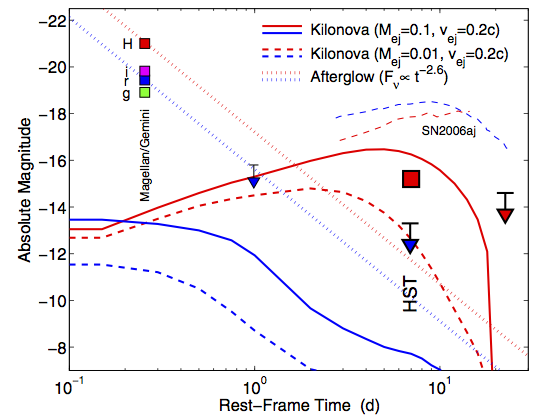
\includegraphics[scale=0.85]{figs/transients/kilonovaBerger.png}
\caption{Kilonova signature in the short GRB\,130603B as revealed by the
Hubble Space Telescope (HST). The Magellan and Gemini telescopes sampled
the optical afterglow of the GRB (dotted lines). The kilonova light
starts to dominate the emission in the H band around a few days after
the merger. Thick and dashed lines: theoretical kilonova models from
\citet{Barnes13} showing that kilonovae are fast-evolving, faint and red
transients. The light-curve of the SN\,2006aj associated with the long
GRB\,060218  is also shown for comparison. From \citet{Berger13}.}
\label{Fig:kilonova}
\end{figure}


% --------------------------------------------------------------------

\subsection{OpSim Analysis and Discussion}
\label{sec:\secname:analysis}

Effective follow up of GW triggers relies on the capability to sample a
relatively large portion of the sky, repeatedly, over a time scale $<1$
week, with different filters \citep{Cowperthwaite15}. In the optical
band, the kilonova signature is expected to be more prominent in the
$i$, $z$  and $y$ filters, which we identify as the most promising
filters for the kilonova search. We emphasize however that another set
of contemporaneous observations in  a ``bluer" filter is necessary to
acquire color information and distinguish kilonovae from other
fast-evolving transients.

We use the median inter-night gap  for visits in the same filter derived
from the candidate Baseline Cadence \texttt{minion\_1016} to show that,
in the absence of a Target of Opportunity (ToO) capability, it is
\emph{not} possible for LSST  to play a major role in the identification
of EM counterparts of GW triggers.

To identify kilonova candidates we need at least 2 observations acquired
within $\sim 1$ week  of the GW event \citep{Cowperthwaite15}. Using the
inter-night gap distribution for visits in the $y$ filter (which is the
most promising filter for a kilonova search), the area of the sky
covered with cadence  $\Delta t<7$ days at any given time, is
$A_{sky}\sim 3000$ deg$^2$ (including deep drilling fields).  This is
the area that can be searched for fast evolving transients.  Two
important considerations follow:

\begin{itemize}
\item[(1)] $A_{sky}$ only covers $P\sim7$\% of the sky. The  probability
that the \emph{entire} GW localization region is contained, by chance,
within $A_{sky}$ is thus very small.
\item[(2)] Even if LSST is able to cover a meaningful portion of the GW
region, we would still not have color information, and we would thus be
unable to filter out contaminating transients.
\end{itemize}

\textbf{We conclude that relying on the serendipitous alignment of the
LSST fields with the GW localization map is not an effective strategy to
follow up GW triggers and identify their EM counterparts. We thus
strongly recommend a ToO capability as part of the baseline LSST
operations strategy.}

Ideally, the ToO capability will allow for imaging of the GW
localization map at least twice over $\Delta t\lesssim$1 week with a
``red" filter ($i$, $z$  or $y$),  and  will include the possibility to
designate a desired set of filters to obtain color information. By the
time of LSST operation the typical size of the GW localization region is
expected to be 10-100 deg$^2$, which would require a small number of
LSST re-pointings. We thus do \emph{not} anticipate a significantly
disruptive impact on other LSST campaigns (especially if only the GW
triggers with the best localizations in the southern sky are selected
for LSST ToOs).

\textbf{At the price of re-shuffling a reasonably small number of
fields, \emph{if} equipped with ToO capabilities, LSST can be the
premier player in the era of EM follow up to GW sources.}

% ====================================================================
%
% \subsection{Conclusions}
%
% Here we answer the ten questions posed in
% \autoref{sec:intro:evaluation:caseConclusions}:
%
% \begin{description}
%
% \item[Q1:] {\it Does the science case place any constraints on the
% tradeoff between the sky coverage and coadded depth? For example, should
% the sky coverage be maximized (to $\sim$30,000 deg$^2$, as e.g., in
% Pan-STARRS) or the number of detected galaxies (the current baseline but
% with 18,000 deg$^2$)?}
%
% \item[A1:] ...
%
% \item[Q2:] {\it Does the science case place any constraints on the
% tradeoff between uniformity of sampling and frequency of  sampling? For
% example, a rolling cadence can provide enhanced sample rates over a part
% of the survey or the entire survey for a designated time at the cost of
% reduced sample rate the rest of the time (while maintaining the nominal
% total visit counts).}
%
% \item[A2:] ...
%
% \item[Q3:] {\it Does the science case place any constraints on the
% tradeoff between the single-visit depth and the number of visits
% (especially in the $u$-band where longer exposures would minimize the
% impact of the readout noise)?}
%
% \item[A3:] ...
%
% \item[Q4:] {\it Does the science case place any constraints on the
% Galactic plane coverage (spatial coverage, temporal sampling, visits per
% band)?}
%
% \item[A4:] ...
%
% \item[Q5:] {\it Does the science case place any constraints on the
% fraction of observing time allocated to each band?}
%
% \item[A5:] ...
%
% \item[Q6:] {\it Does the science case place any constraints on the
% cadence for deep drilling fields?}
%
% \item[A6:] ...
%
% \item[Q7:] {\it Assuming two visits per night, would the science case
% benefit if they are obtained in the same band or not?}
%
% \item[A7:] ...
%
% \item[Q8:] {\it Will the case science benefit from a special cadence
% prescription during commissioning or early in the survey, such as:
% acquiring a full 10-year count of visits for a small area (either in all
% the bands or in a  selected set); a greatly enhanced cadence for a small
% area?}
%
% \item[A8:] ...
%
% \item[Q9:] {\it Does the science case place any constraints on the
% sampling of observing conditions (e.g., seeing, dark sky, airmass),
% possibly as a function of band, etc.?}
%
% \item[A9:] ...
%
% \item[Q10:] {\it Does the case have science drivers that would require
% real-time exposure time optimization to obtain nearly constant
% single-visit limiting depth?}
%
% \item[A10:] ...
%
% \end{description}

% ====================================================================

\navigationbar


% --------------------------------------------------------------------

% ====================================================================
%+
% SECTION:
%    grb.tex  % eg lenstimedelays.tex
%
% CHAPTER:
%    transients.tex  % eg cosmology.tex
%
% ELEVATOR PITCH:
%    Explain in a few sentences what the relevant discovery or
%    measurement is going to be discussed, and what will be important
%    about it. This is for the browsing reader to get a quick feel
%    for what this section is about.
%
% COMMENTS:
%
%
% BUGS:
%
%
% AUTHORS:
%    Phil Marshall (@drphilmarshall)  - put your name and GitHub username here!
%-
% ====================================================================

\section{Gamma-Ray Burst Afterglows}
\def\secname{grbs}\label{sec:\secname} % For example, replace "keyword" with "lenstimedelays"

\credit{ebellm} % (Writing team)

Gamma-ray bursts (GRBs) are relativistic explosions typically classified by the temporal duration of their initial gamma-ray emission: Long GRBs, that mark the endpoint of the lives of some massive stars, and short GRBs, believed to originate from the merger of binary neutron stars.
GRB emission is known to be beamed: the initial prompt gamma-ray emission is seen only for observers looking at the jet axis. The longer-wavelength X-ray, optical, and radio afterglow may be seen both by on- and off-axis observers.  The latter case is known as an orphan afterglow, due to the absence of gamma-ray emission.  
On- and off-axis afterglows are predicted to have different temporal signatures in the optical: On-axis events decay as a power-law until a jet break, while off-axis events should be fainter and show an initial rise 
Despite systematic searches, no convincing orphan afterglow candidates have yet been discovered, limiting our knowledge of the beaming fraction of GRBs and hence their true rates.
Well-sampled orphan afterglow lightcurves would also permit study of the GRB 
jet structure.

Because of their rarity, in all but one case \citep{2015ApJ...803L..24C} to date GRBs have been discovered using their prompt emission by hard X-ray or gamma-ray all-sky monitors.  
This selection imposes biases on the population of relativistic explosions we observe.  
Baryon-loading in the GRB jet---a ``dirty fireball'' \citep{2003ApJ...591.1097R}---can lead to on-axis events without gamma-ray emission.  Only one plausible candidate has been identified to date \citep{2013ApJ...769..130C}.  
Discovery of new dirty fireballs---if distinguished from off-axis events--would clarify the rates of these events and enhance our understanding of the diversity of stellar death.

LSST is the survey most capable of resolving these decades-old questions.  Due to its large aperture and etendue, LSST can detect faint, fast-fading, and rare cosmological events, potentially enabling population studies of the high-redshift universe.  
\citet{2015A&A...578A..71G} estimated LSST could detect 50 orphan afterglows each year, more than any other planned survey.

%deep survey helps due to time dilation

%beaming fraction and true rates; jet structure; dirty fireballs?
%GRB-SN connection; probe high-z star formation?

%other fast transients: Fast transients and SN shock breakout?  flash spectroscopy

% --------------------------------------------------------------------

\subsection{Target measurements and discoveries}
\label{sec:\secname:targets}

GRB afterglow discovery is among the science cases that places the greatest stress on the LSST cadence.  Because afterglows fade rapidly---dropping several magnitudes in the first few hours---high cadence observations are required to detect the fast fading.  
If an afterglow candidate can be recognized in real time, it will be possible to trigger TOO spectroscopy (to measure a redshift and confirm the event is cosmological), X-ray observations (to detect a high-energy counterpart), and additional photometry (to characterize the lightcurve evolution).  If there is no source at the location of the transient in the coadded reference image, two consecutive observations in the same filter separated by an hour or two are the minimum required to potentially trigger followup of a fast-fading event.  
However, a third or fourth observation in a single night---ideally in the same filter---would improve the purity of the sample.  Observations in other bands at high cadence are less useful because they require assumptions about the event's SED and its evolution to determine if a source is truly fading.

Distinguishing orphan afterglows from on-axis events (whether conventional GRBs or dirty fireballs) will also require more than two detections.  Orphan events may prove harder to recognize in real time, because they are intrinsically fainter than on-axis events and show an initial rise rather than a rapid decay.  
Additionally, because of relativistic time dilation high redshift events are easier to detect, but these events will be fainter and more difficult to follow up.
Accordingly, population studies of orphan afterglow candidates may be best conducted with LSST photometry alone.  These may only be productive if LSST has suffiently frequent revisits to a field in a single filter.


% --------------------------------------------------------------------

\subsection{Metrics}
\label{sec:\secname:metrics}

The core figure of merit for GRB afterglows is simply the raw number of on- and off-axis events detectable in two, three, or more observations, preferably in a single filter.

The appropriate way to derive these detections is to conduct a Monte Carlo simulation of a cosmological population of GRBs and fold it through the LSST observing cadence \citep[cf.][]{2011PASP..123.1034J}.  We are pursuing developing this infrastructure in the MAF framework.  

Simplified metrics can give us a general idea of how well a given cadence can characterize fast-evolving transients such as GRBs.


% --------------------------------------------------------------------

\subsection{OpSim Analysis}
\label{sec:\secname:analysis}

OpSim analysis: how good would the default observing strategy be, at
the time of writing for this science project?


% --------------------------------------------------------------------

\subsection{Discussion}
\label{sec:\secname:discussion}

Discussion: what risks have been identified? What suggestions could be
made to improve this science project's figure of merit, and mitigate
the identified risks?


% ====================================================================

\navigationbar


% --------------------------------------------------------------------
